%\documentclass[aspectratio=43]{beamer} %4:3 ratio presentatie
\documentclass[aspectratio=169]{beamer} %16:9 ratio presentatie


\usetheme[]{default}
\usecolortheme{beaver}
\usepackage{tikz}
\usepackage{multirow}
\usepackage{xcolor}
\usepackage{graphicx}

\beamertemplatenavigationsymbolsempty %suppress navigation bar
\definecolor{light-gray}{gray}{0.1}
%\addtobeamertemplate{frametitle}{}

%TITLEPAGE
\title[Imputing squares] {Predictive Ratio Matching Imputation\\ {\small of Nested Compositional Data with Semicontinuous Variables}}
%\author[Vink, Van Buuren]
%{
%  Gerko~Vink\inst{1,2} \and
%  Stef~Van Buuren\inst{1,3} \and
%}
%
%\institute[Utrecht University and others]
%{
%  \inst{1}%
%  Utrecht University
%  \and
%  \vskip-2mm
%  \inst{2}%
%  Statistic Netherlands
%  \and
%  \vskip-2mm
%  \inst{3}%
%  Netherlands Organization for Applied Scientific Research TNO
%  \vskip6mm
%}

\author[Vink, Pannekoek, Van Buuren]
{
  Gerko~Vink \and
  Jeroen~Pannekoek \and
  Stef~van Buuren
}


\date[ISA 2014]
{\vspace{.5 in}\\JSM 2014 \vskip6mm}



\begin{document}

%%%%
%\begin{frame}
\titlepage
\begin{tikzpicture}[remember picture,overlay]
\node[anchor=south, yshift=2pt] at (current page.south) {
\includegraphics[height=0.8cm] {UU.png} 
\includegraphics[height=0.8cm]{TNO.png} 
\includegraphics[height=0.8cm]{CBS.png}\hspace{.25 in}};
\end{tikzpicture}
%\end{frame}

%%%%
\begin{frame}
  \frametitle{COMPOSITIONAL DATA}
Let us consider $x_0$ as a combination of $x_1$ through $x_D$, such that
\begin{equation*}
\label{eq1}
x_0=x_1+x_2+...+x_D,
\end{equation*}
where the integers $1,2,...,D$ denote the parts and the subscripted letters $x_1, ...,x_D$ denote the components.
 \end{frame}

\begin{frame}
  \frametitle{SOME MORE BACKGROUND}
All the information about compositional data is encapsulated in the ratios between the components\footnote{\tiny{Aitchison, J. (1986). \emph{The statistical analysis of compositional data}. Chapman \& Hall.}}. Consequently, the proportions of the different parts of $x$ obey 
\begin{equation*}
\label{eq2}
\frac{x_1}{x_0}+\frac{x_2}{x_0}+...+\frac{x_D}{x_0}=1,
\end{equation*}
where
\begin{equation*}
\label{eq3}
x_1\geq0,x_2\geq0,...,x_D\geq0,
\end{equation*}
such that the sample space is defined as simplex $S^D$
\begin{equation*}
S^D = \{(x_1,x_2,\dots,x_D) : x_j \geq 0;j = 1,2,\dots,D;\sum_{j}^{D}x_j = x_0\}.
\end{equation*}
\end{frame}

\begin{frame}
  \frametitle{MISSINGS IN A SINGLE COMPOSITION}

\begin{equation*}
\label{top}
x_0=\textcolor{red}{x_1}+\textcolor{red}{x_2}+x_3
\end{equation*}
\begin{equation*}
\textcolor{red}{x_1}+\textcolor{red}{x_2}=x_0-x_3
\end{equation*}
We can solve this by imputing the ratio $\pi = x_2/(x_1+x_2)$ from a probable donor record $d$, yielding\begin{equation*}
x_1^*=\pi^*_{(21)}(x_0-x_3), 
\end{equation*}
and its complement
\begin{equation*}
x_2^*=(1-\pi^*_{(21)})(x_0-x_3),
\end{equation*}
where ${\pi^*_{21}}$ is the imputed ratio for pair $21$ and comes from the distribution
\begin{equation*}
\Pr(\pi^*_{21}|\pi_{21}, x_{0}, x_{3})
\end{equation*}
of donors with both $x_2$ and $x_1$ observed. 
\end{frame}

\begin{frame}
  \frametitle{MULTIVARIATE MISSINGS IN A SINGLE COMPOSITION}

\begin{equation*}
\label{top}
x_0=\textcolor{red}{x_1}+\textcolor{red}{x_2}+\textcolor{red}{x_3}+x_4
\end{equation*}
\begin{equation*}
\textcolor{red}{x_1}+\textcolor{red}{x_2} + \textcolor{red}{x_3}=x_0-x_4
\end{equation*}
We can solve this by finding starting values for $x_1$, $x_2$ and $x_3$ and iteratively updating the bivariate ratios from probable donor records.
\newline \\
Any starting value will be sufficient as long as the compositional structure
remains intact.
\newline \\
All ${j \choose 2}$ unique pairs, where $j$ is the number of variables can be imputed by means of this approach and variables outside of the currently imputed pair, as well as the total of the composition, can serve as covariates in the prediction of $\pi^*$.
\end{frame}

\begin{frame}
  \frametitle{MULTIVARIATE MISSINGS IN A SINGLE COMPOSITION}
\begin{equation*}
\label{top}
x_0=\textcolor{red}{x_1}+\textcolor{red}{x_2}+\textcolor{red}{x_3}+x_4
\end{equation*}
The ${j \choose 2}$ unique pairs in the above problem are
\begin{equation*}
\begin{array}{cc}
x_1 &x_2\\
x_1 &x_3\\
x_1 &x_4\\
x_2 &x_3\\
x_2 &x_4\\
x_3 &x_4\\
\end{array}
\end{equation*}
\end{frame}

\begin{frame}
  \frametitle{MULTIVARIATE MISSINGS IN A SINGLE COMPOSITION}
Some pairs do not need updating, as $x_4$ is observed and we would not want to alter observed values. 
\begin{equation*}
\begin{array}{cc}
\textcolor{red}{x_1} &\textcolor{red}{x_2}\\
\textcolor{red}{x_1} &\textcolor{red}{x_3}\\
x_1 &x_4\\
\textcolor{red}{x_2} &\textcolor{red}{x_3}\\
x_2 &x_4\\
x_3 &x_4\\
\end{array}
\end{equation*}
Missings in pairs where one of the variables is observed will be imputed in another pair where both variables are missing (if only one variable is missing, the equation could have been solved deductively)
\newline \\
Only having to consider jointly missing pairs makes PRM much faster. 
\end{frame}

\begin{frame}
  \frametitle{PRM APPROACH}
We require that starting values have been filled in and that any deductive imputation has been applied.
\newline \\
Carry out the following steps for all ${j \choose 2}$ unique pairs (\textcolor{red}{simplified version}).
\begin{enumerate}
	\item Calculate $\pi^{obs}$ (if not defined: $\pi^{obs} = 0.5$). 
	\item Impute $\pi^{mis}$ 
	\item Redistribute amounts
\end{enumerate}
Repeat the above algorithm until convergence is reached. For multiple imputation do this $m\geq2$ times
\newline \\
Imputations could be obtained by e.g. PMM with $\pi^{obs}$ conditional on the remaining variables and the total.		
\end{frame}

%
%\begin{frame}
%PRM APPROACH
%\newline \\
%We require that starting values have been filled in and that any deductive imputation has been applied.
%\newline \\
%Carry out the following steps for all ${j \choose 2}$ unique pairs.
%\begin{enumerate}
%	\item Calculate $\pi^{obs}$ and replace all $\pi^{obs}$ that are not defined (when both variables are 0) with $\pi^{obs} = 0.5$. 
%	\item Impute $\pi^{mis}$ by means of e.g. PMM with $\pi^{obs}$ conditional on the remaining variables and the total.		
%	\item For all joint missings in the pair, redistribute the sum of that pair over the variables in the pair
%\end{enumerate}
%Repeat the above algorithm until convergence is reached. For multiple imputation do this $m\geq2$ times, preferably in parallel with different random seeds, each time saving the completed dataset. 
%\end{frame}

\begin{frame}
\huge
\begin{equation*}
\begin{array}{cccc}
x_0 &x_1   & x_2  & x_3    \\
32 	&10   & 15  	& 7	\\
18 	&0	&9		&9	\\
22 	&6	& 3		& -	\\
14 	&0	&-		&-	\\
8	&22	&-		&4	\\
30 	&-	&-		&-	\\
\end{array}
\end{equation*}
\end{frame}  
  
\begin{frame}
  \frametitle{BENEFITS OF PRM}
By addressing the ratios between pairs, the compositional problem can be solved outside the simplex space
\newline \\
No need for post-hoc fixes when components are 0
\newline \\
The flexibility of imputation by chained equations - (m)ice

\end{frame}

\begin{frame}
  \frametitle{NESTED COMPOSITIONS: UNOBSERVED NESTED SUM}
Suppose that we have a nested composition, where $x_4$ is a combination of $x_5$ and $x_6$, such that
\begin{equation*}
x_4=x_5+x_6.
\end{equation*}
For the cases where $x_4$ is missing, the problem can be simplified to 
\begin{equation*}
x_1=x_2+x_3+x_5+x_6,
\end{equation*}
where $x_4$ can be deductively calculated after $x_5$ and $x_6$ are imputed. 
\newline \\
This reduces the problem to a single composition, which can easily be solved by the proposed PRM algorithm.
\end{frame}

\begin{frame}
  \frametitle{NESTED COMPOSITIONS: OBSERVED NESTED SUM}
For the cases where $x_4$ is observed,  the problem can be divided into the independent imputation problems 
\begin{equation*}
x_1=x_2+x_3+x_4\quad \textnormal{and}\quad x_4=x_5+x_6.
\end{equation*} 
Solving these separate compositions is also straightforward with the proposed PRM algorithm.
\newline \\
In both cases donors are drawn from within the compositional level of the missing values. 
\end{frame}

\begin{frame}
  \frametitle{MISSINGS IN MULTIPLE NESTED COMPOSITIONS}
\begin{equation*}
\begin{array}{lllllllllllll}
x_0 &=	&x_1		&+	&x_2		&+		&x_3		&+& x_4	& 		& 	& 	&\\
       &  	&= 		&   	&      		& 		&  		&& =		& 		& 	&	&\\
       &  	&x_9    	&   	&      		&		& 		&& x_5	& 		& 	&	&\\
       &  	&+		&   	&      		&		& 		&& +		& 		& 	&	&\\
       &  	&x_{10} 	&   	&      		&		& 	 	&&x_6		&= 		&x_7 	&+&x_8
\end{array}
\end{equation*}

A solution for this data where $x_1$, $x_4$ and $x_6$ are known is simply the summation of a sumscores respective parts, such that
\begin{align*}
x_0 &= x_1 + x_2 + x_3 + x_4\\
x_1 &= x_9 + x_{10} \\
x_4 &= x_5 + x_6\\
x_6 &= x_7 + x_8
\end{align*}
\end{frame}

\begin{frame}
  \frametitle{MISSINGS IN MULTIPLE NESTED COMPOSITIONS}
For unknown $x_6$, all components from $x_6=x_7+x_8$ are moved to the higher level, such that
\begin{align*}
x_0 &= x_1 + x_2 +x_3 + x_4\\
x_1 &= x_9 + x_{10}\\
x_4 &= x_5 + x_7 + x_8.
\end{align*}
For unknown $x_4$ and $x_6$ it holds that
\begin{align*}
x_0 &= x_1 + x_2 +x_3 + x_5 + x_7 + x_8\\
x_1 &= x_9 + x_{10},\\
\end{align*}
and for unobserved $x_1$, $x_4$ and $x_6$ there remains one composition to be imputed, namely
\begin{align*}
x_0 &= x_9 + x_{10} + x_2 +x_3 + x_5 + x_7 + x_8.\\
\end{align*}
\end{frame}

\begin{frame}
  \frametitle{DIVIDE AND CONQUER APPROACH}
Any set of nested compositions can be imputed by means of the following scheme (\textcolor{red}{highly simplified!}). 
\newline \\
Start with the lowest level composition and carry out for all (nested) compositions
\begin{enumerate}
\item For cases where the sumscore of a nested composition is missing
	\begin{enumerate}
	\item Promote the missingness problem to the next higher level composition and save it for later. 
	\end{enumerate}
\item For cases where the sumscore of a nested composition is observed
	\begin{enumerate}
	\item Impute the missing parts in the composition by means of PRM.
	\item Calculate unobserved nested totals (if any) in the current composition based on the imputed parts.
	\end{enumerate}
\end{enumerate}
Repeat the above until convergence is reached. For multiple imputation do this $m\geq2$ times

\end{frame}

\begin{frame}
  \frametitle{EVALUATING PRM}
Simulation study: Dutch Wholesaler Data (DWD) for 2007. The DWD dataset contains edited information on 1067 wholesalers for a set of cost statistics ($a$, $e$, $g$ and $h$) that sum op to a set total $x_0$, leading to composition
\begin{equation*}
x_0=a+e+g+h,
\end{equation*}
\begin{equation*}
\begin{array}{llll}
x_0 &\textnormal{the total operating costs}&&\\
a &\textnormal{company depreciation} &\textnormal{single measure}&\\
e &\textnormal{buying costs} &\textnormal{5 parts}&\\
g &\textnormal{personnel costs} &\textnormal{9 parts}&\\
h &\textnormal{other costs}  &\textnormal{21 parts} &\textnormal{ $h_1=h_2+h_3+h_4$}\\
\end{array}
\end{equation*}
\newline \\
3 missingness mechanisms: left-tailed MAR, right-MAR and MCAR
\end{frame}

\begin{frame}
%  \vspace{ in} %Control vertical offset
  \centering
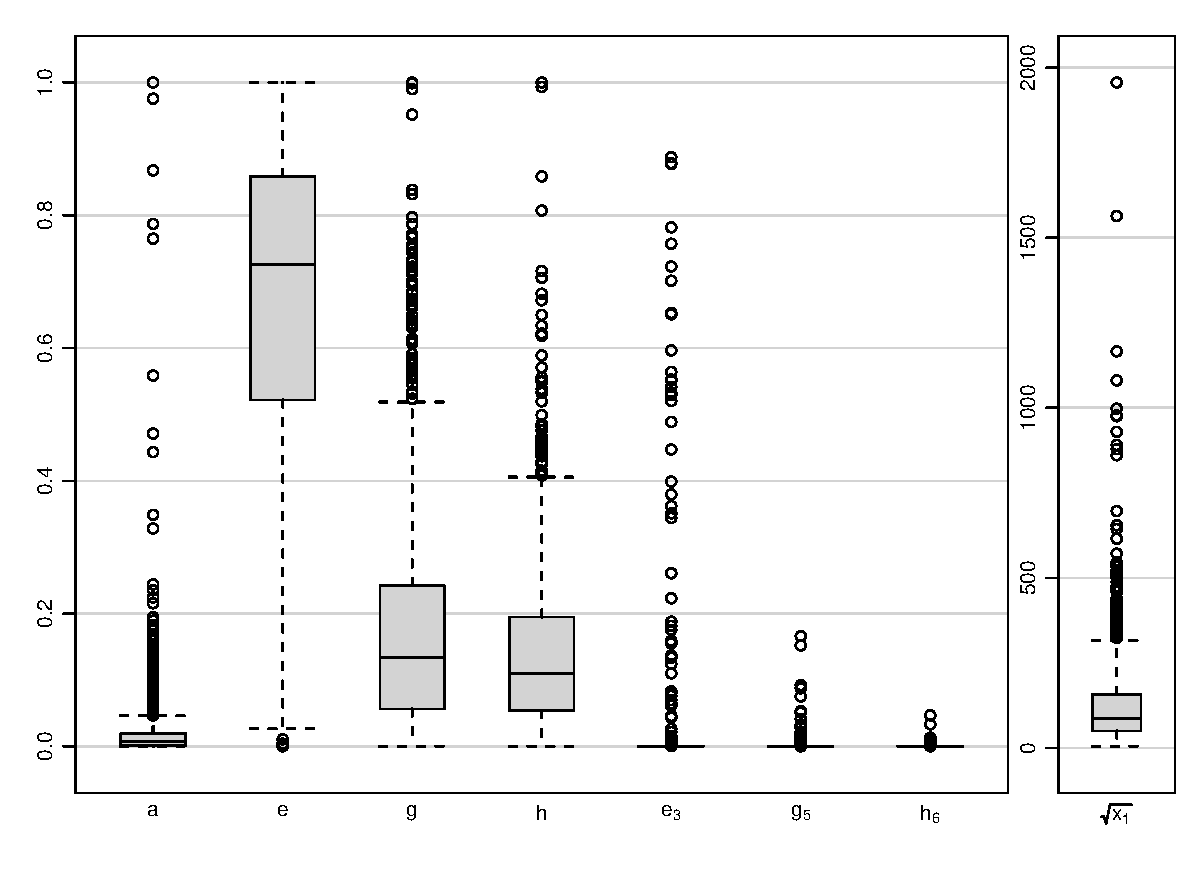
\includegraphics[scale=.55]{bwplot.pdf}
 \end{frame}
 
 \begin{frame}
   \frametitle{15 \% Missingness (27.75 \% bivariate MCAR)}
%  \vspace{-.45 in} %Control vertical offset
  \centering
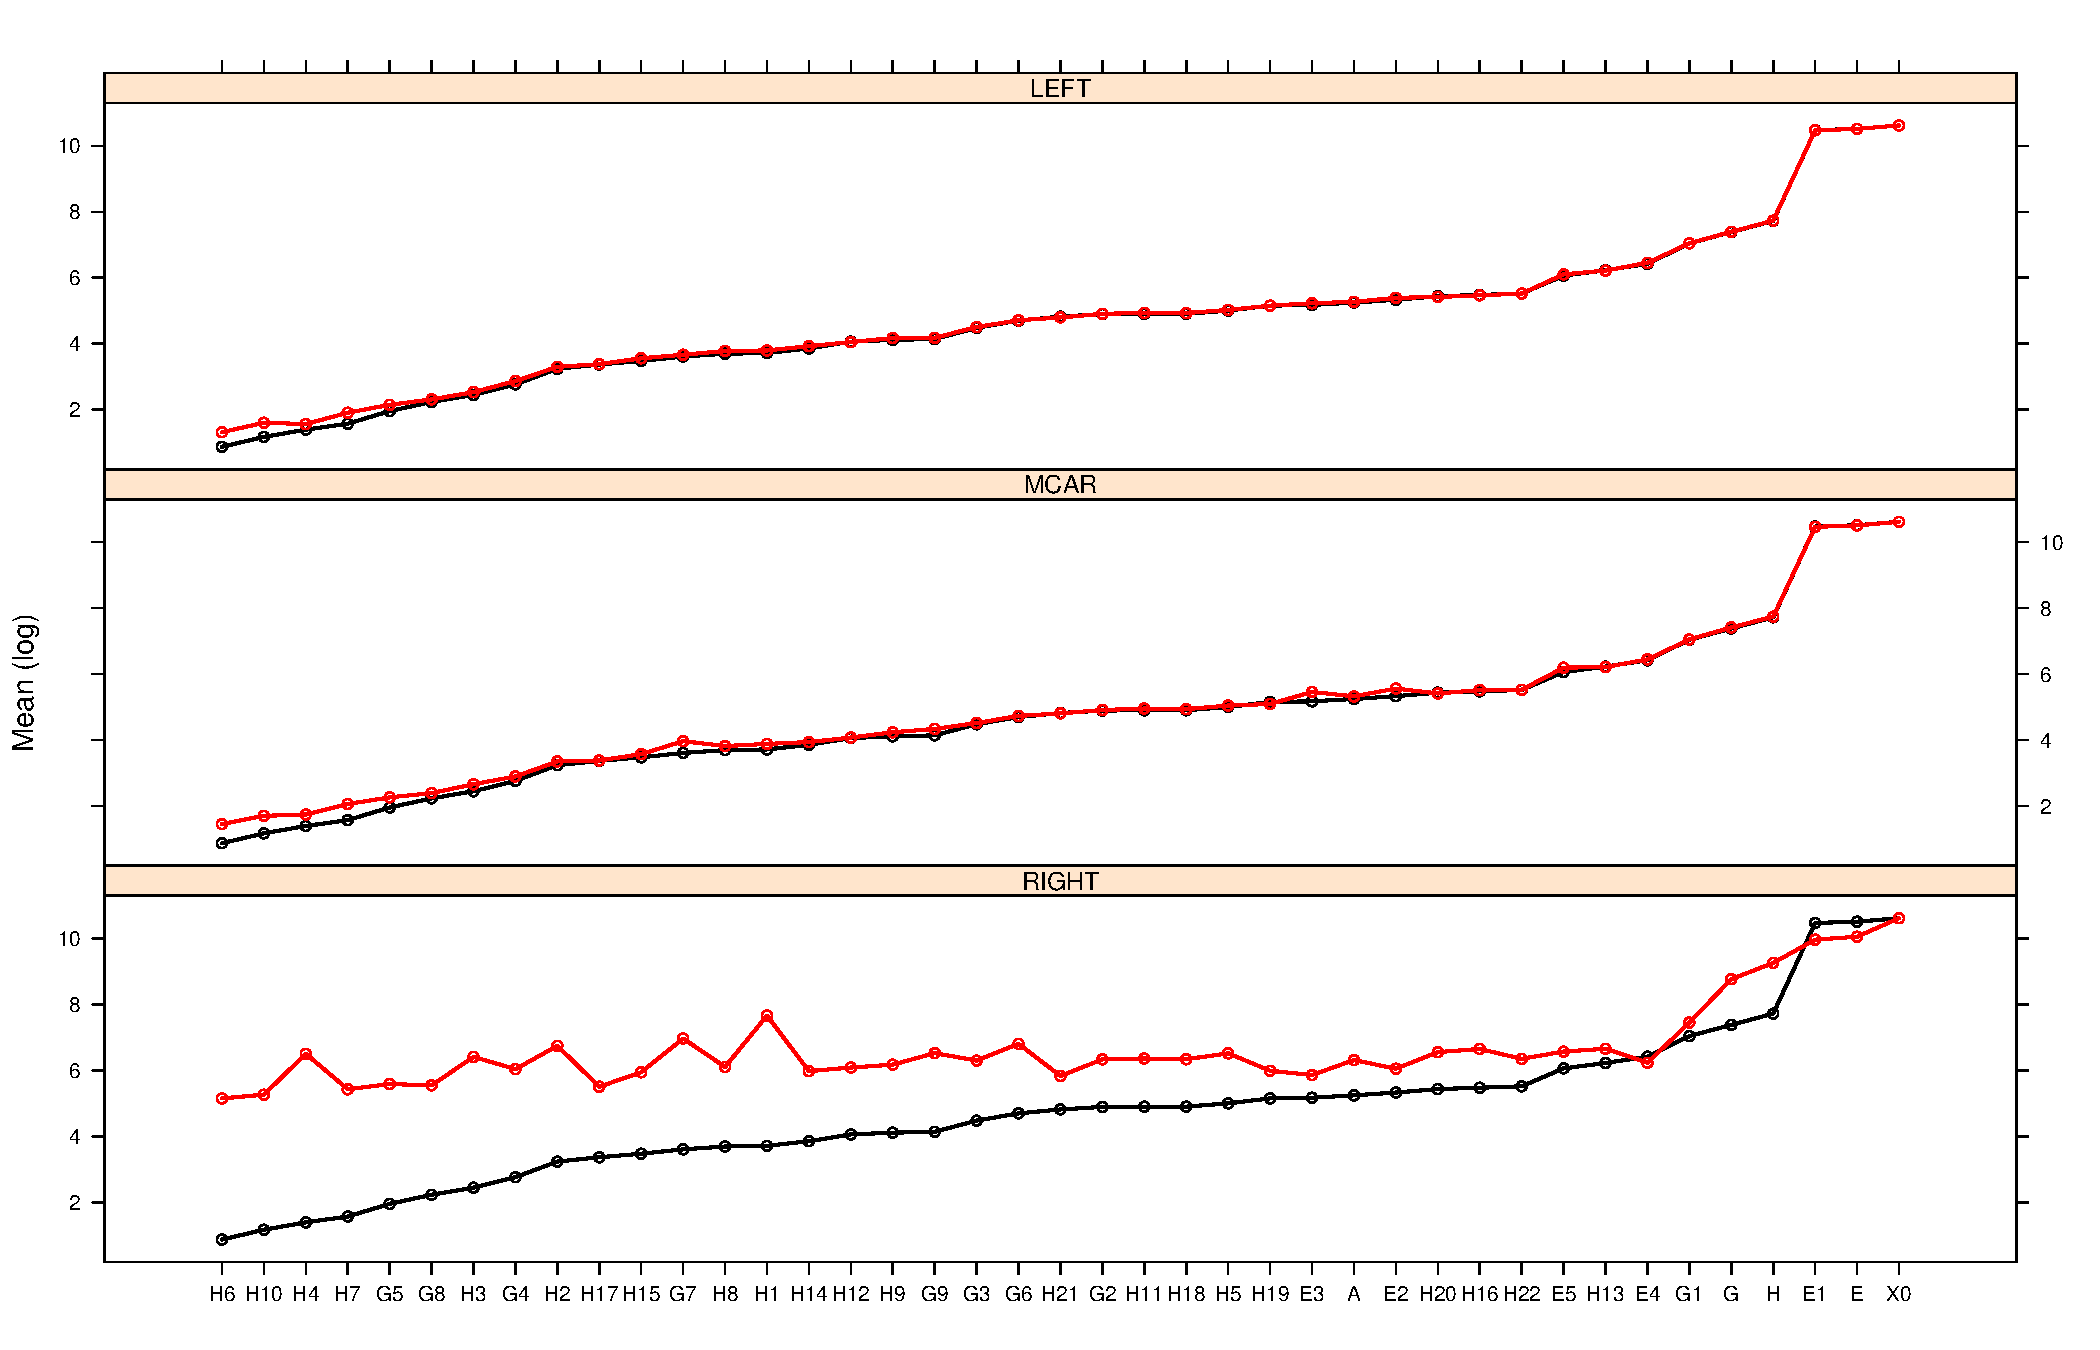
\includegraphics[scale=.3]{plot15.pdf}
 \end{frame}
 
  \begin{frame}
     \frametitle{25 \% Missingness (43.75 \% bivariate MCAR)}
 % \vspace{-.45 in} %Control vertical offset
  \centering
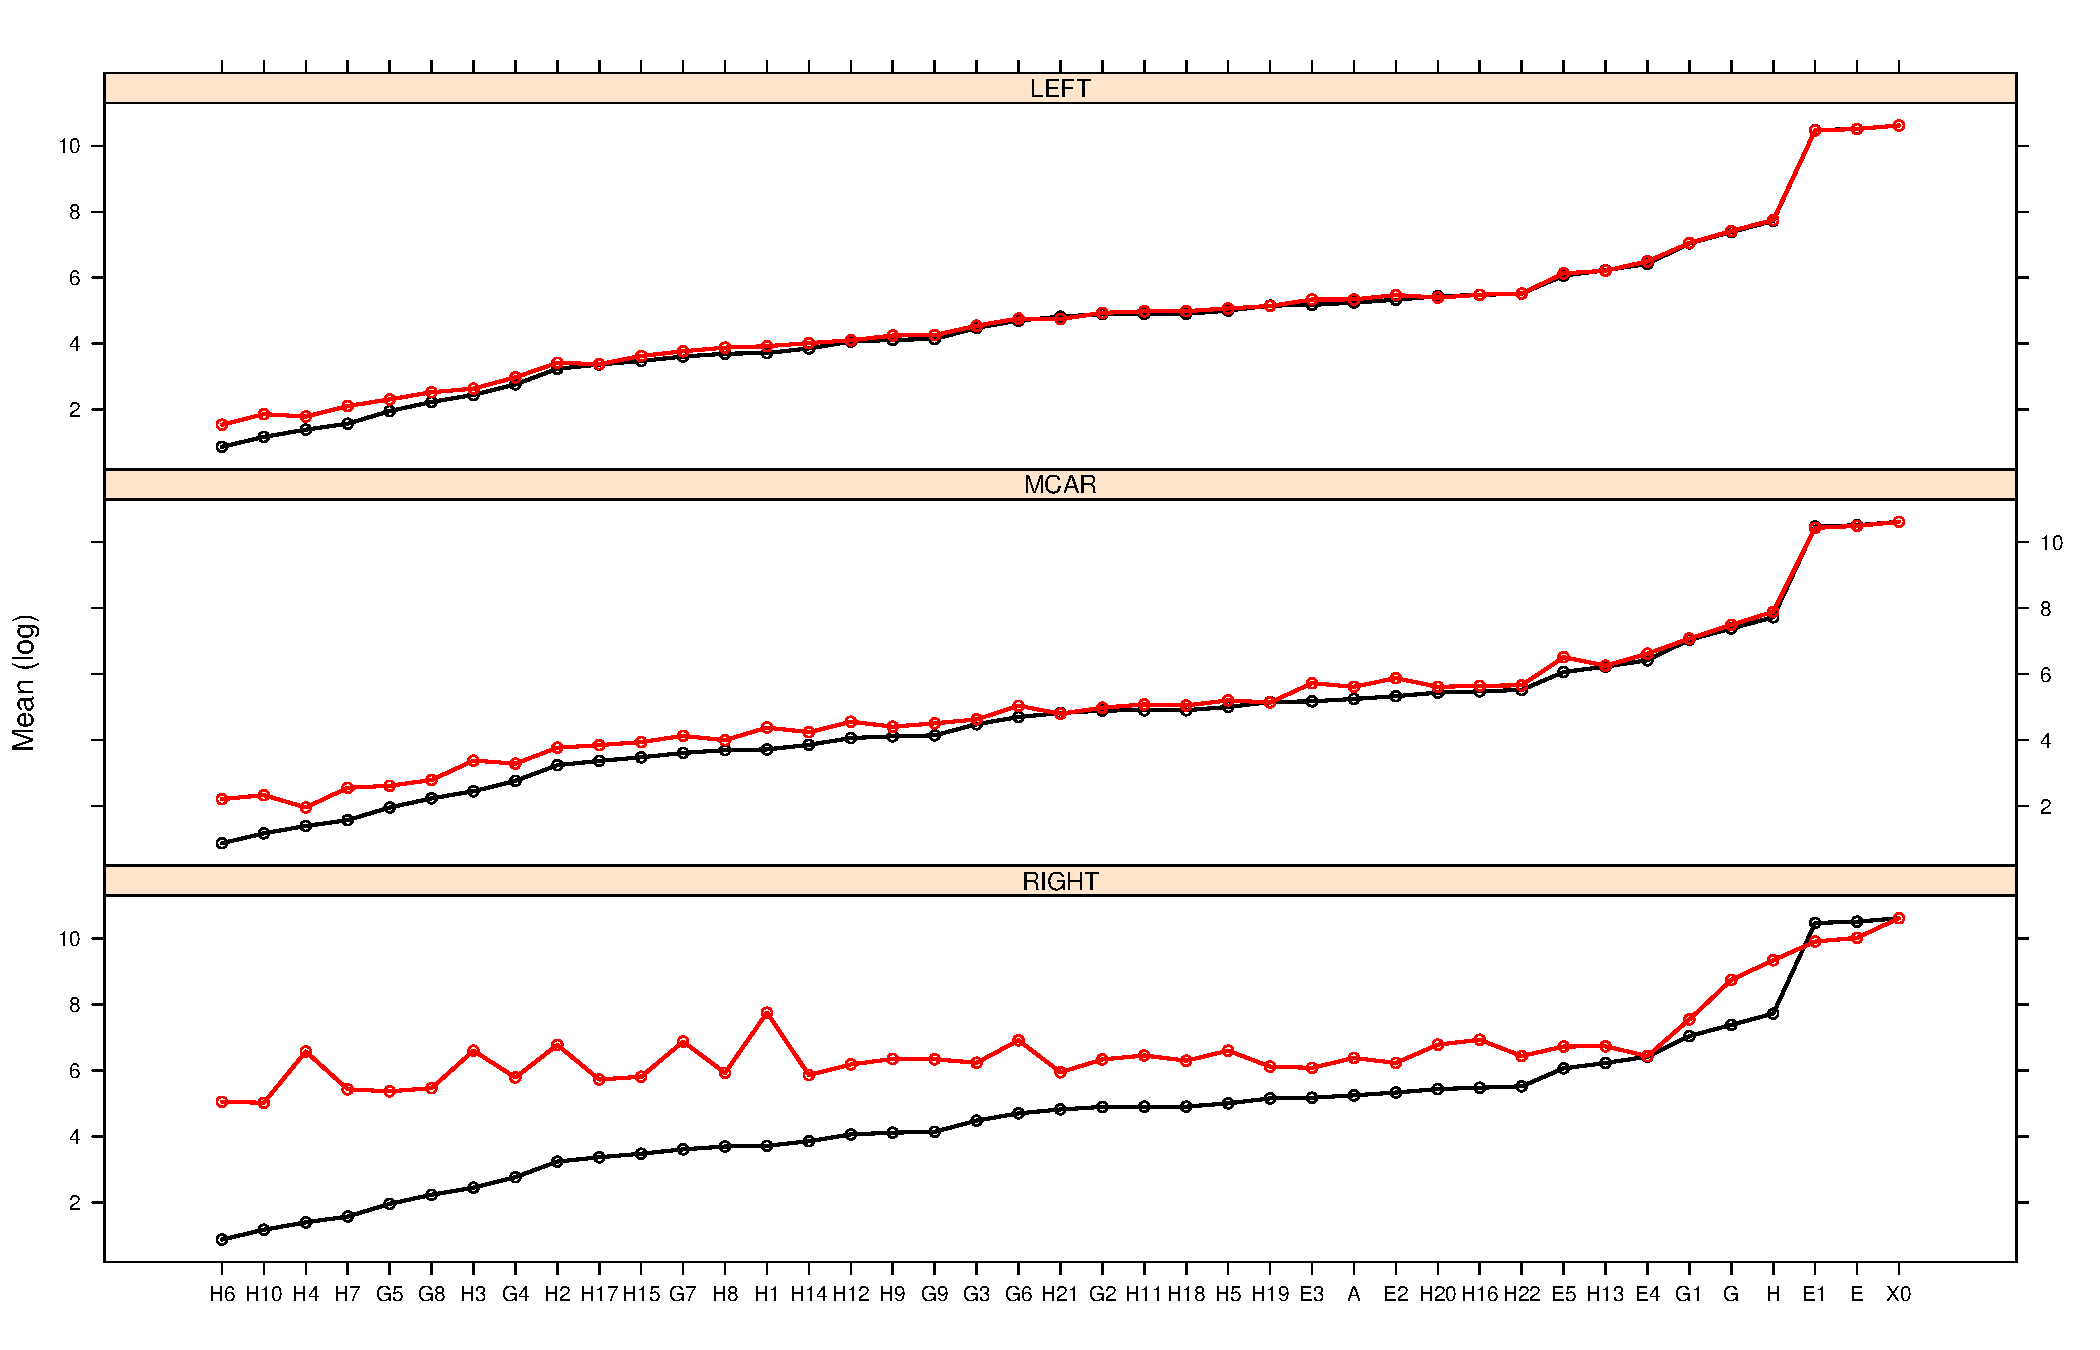
\includegraphics[scale=.3]{plot25.pdf}
 \end{frame}
 
  \begin{frame}
%  \vspace{-.45 in} %Control vertical offset
  \centering
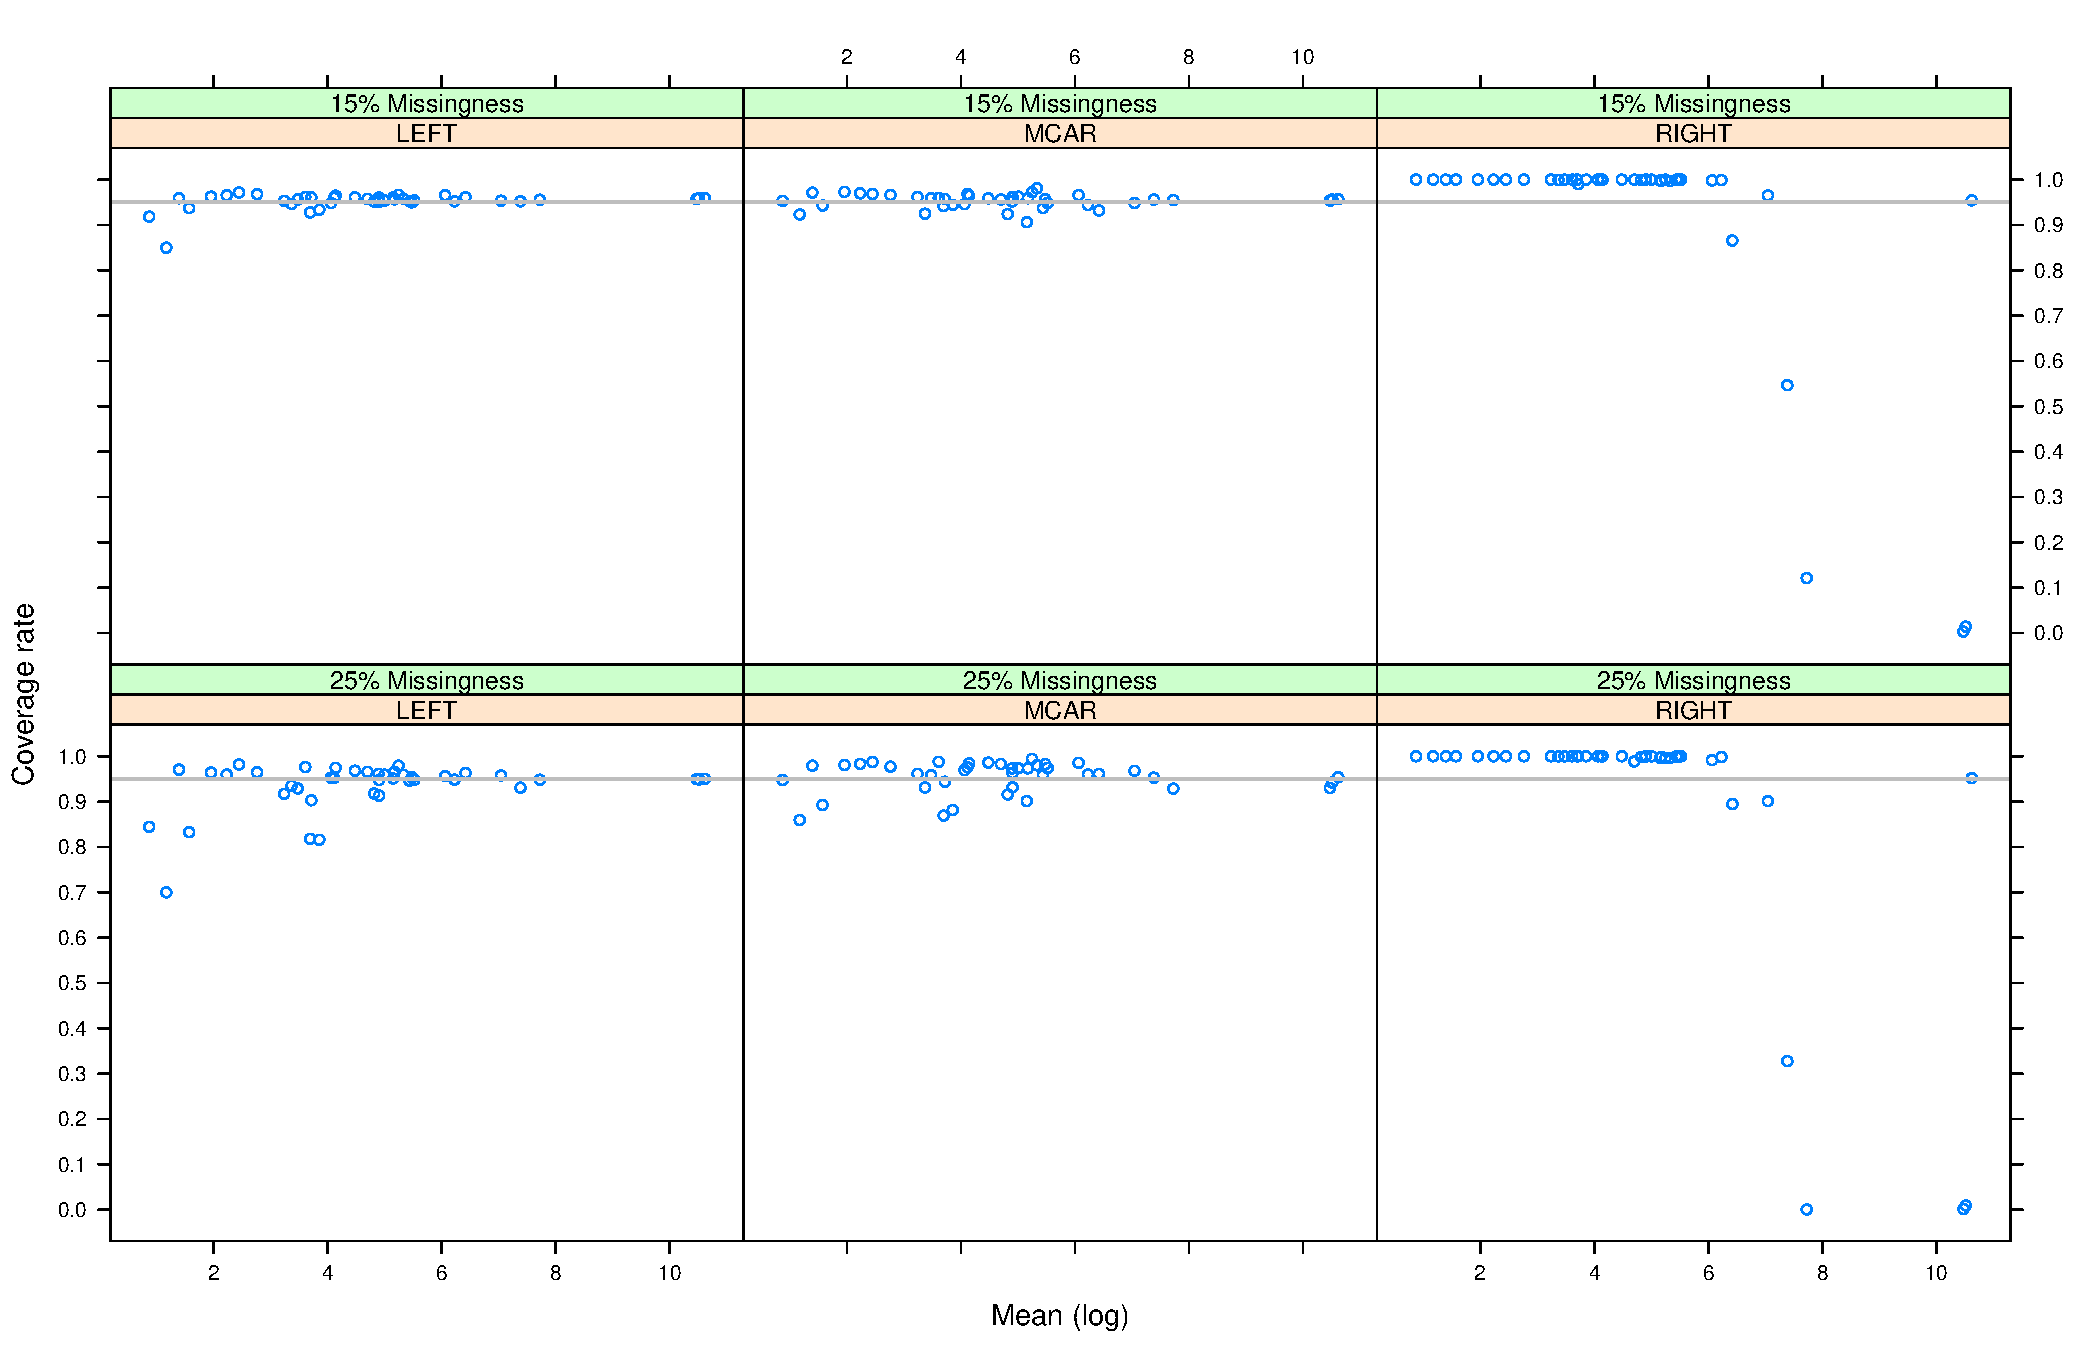
\includegraphics[scale=.3]{plotcov.pdf}
 \end{frame}
 
  \begin{frame}
%  \vspace{-.45 in} %Control vertical offset
  \centering
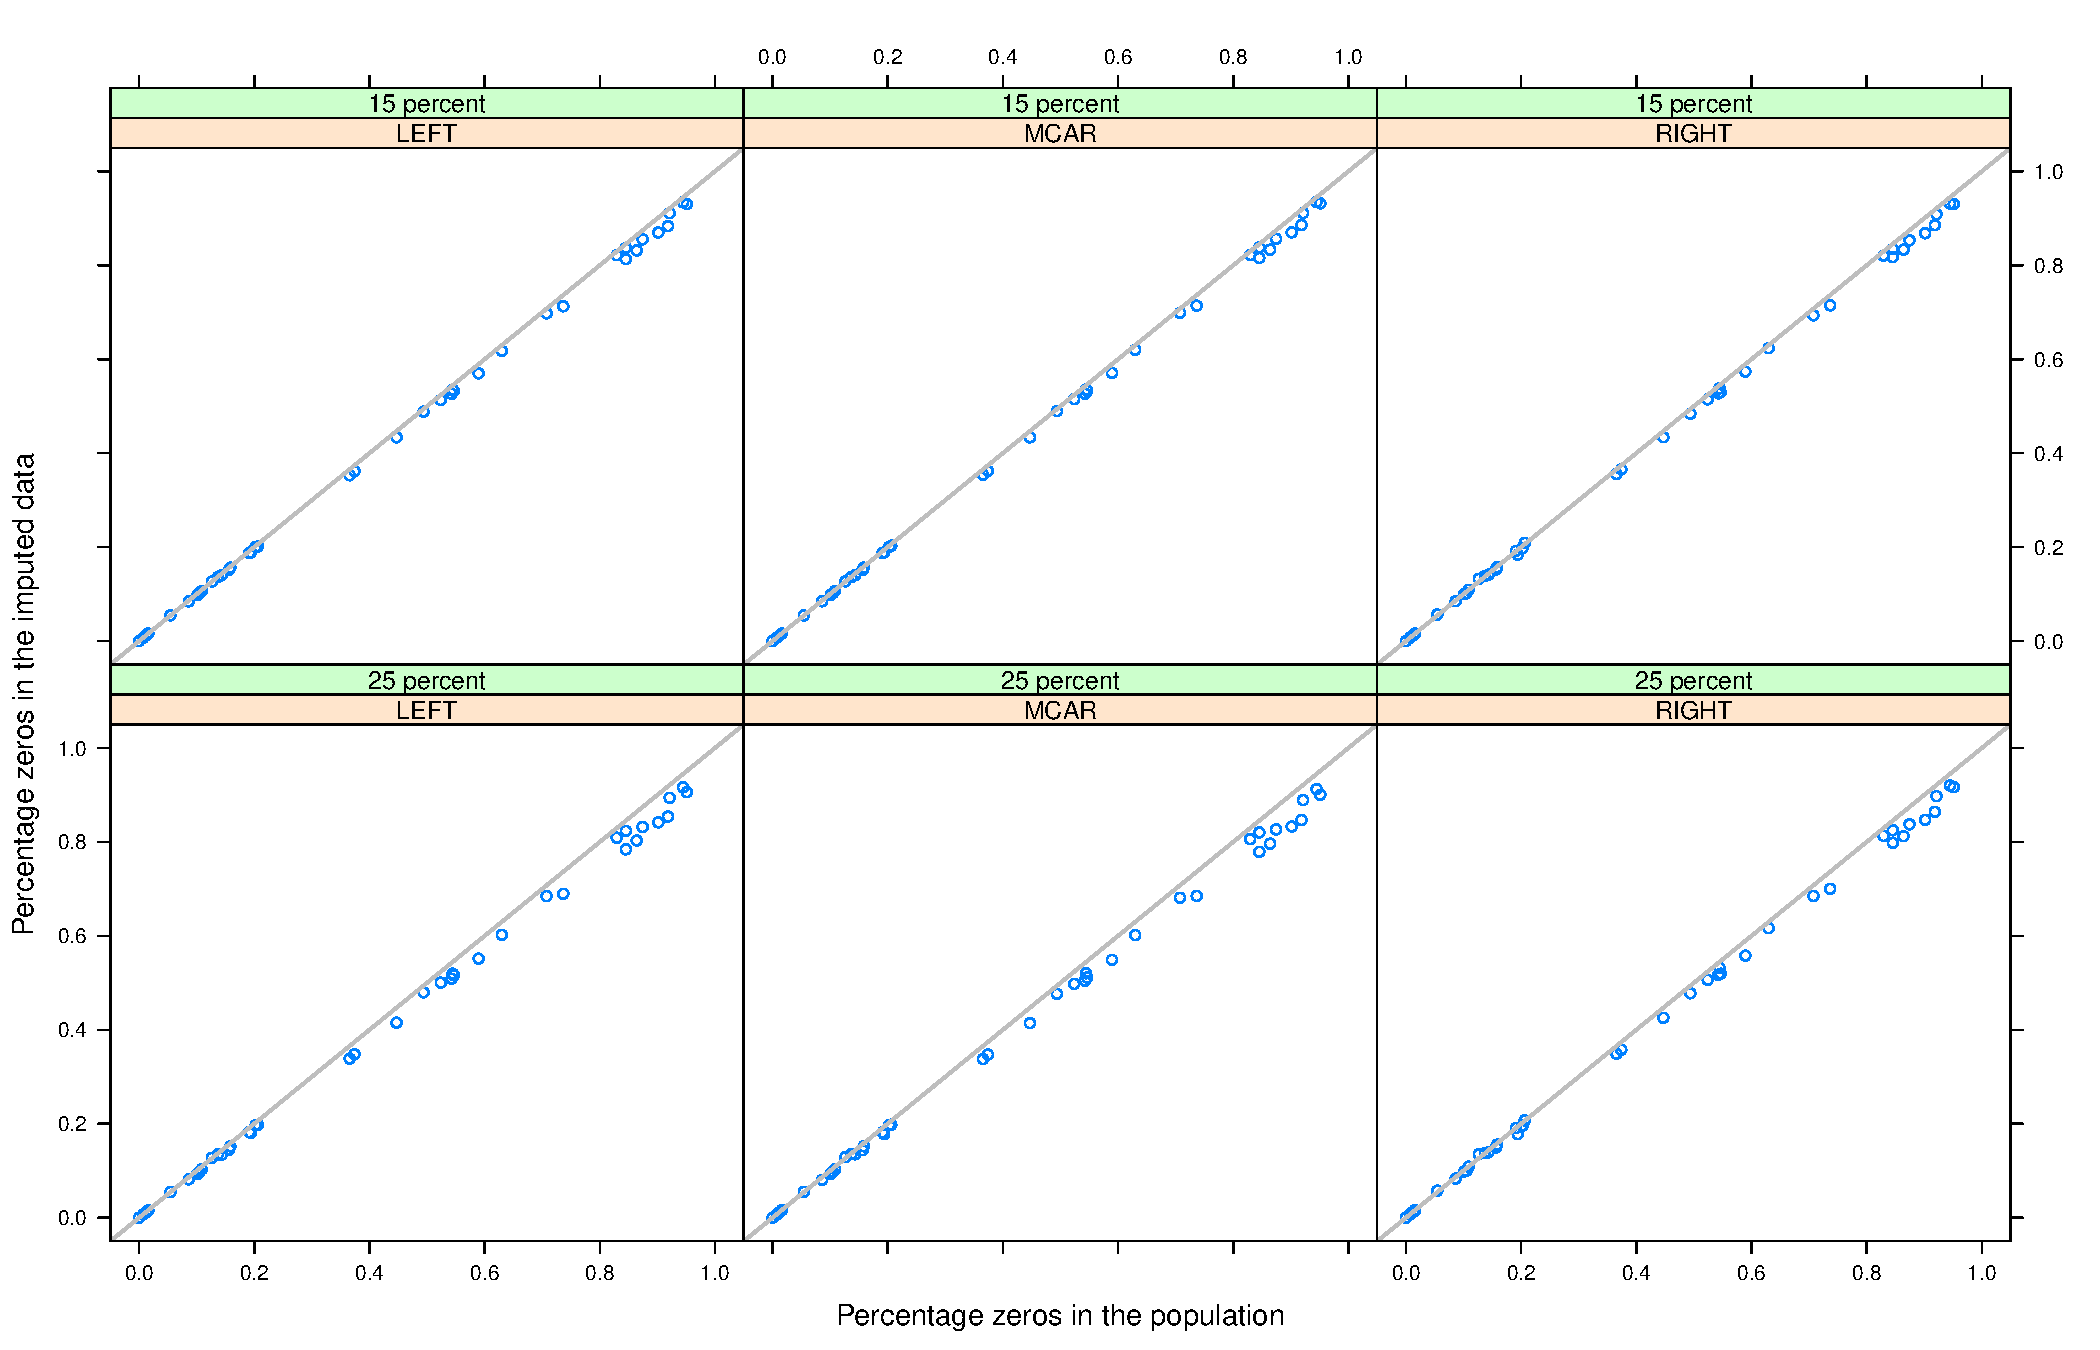
\includegraphics[scale=.3]{plotzero.pdf}
 \end{frame}
 
  \begin{frame}
 % \vspace{-.45 in} %Control vertical offset
  \centering
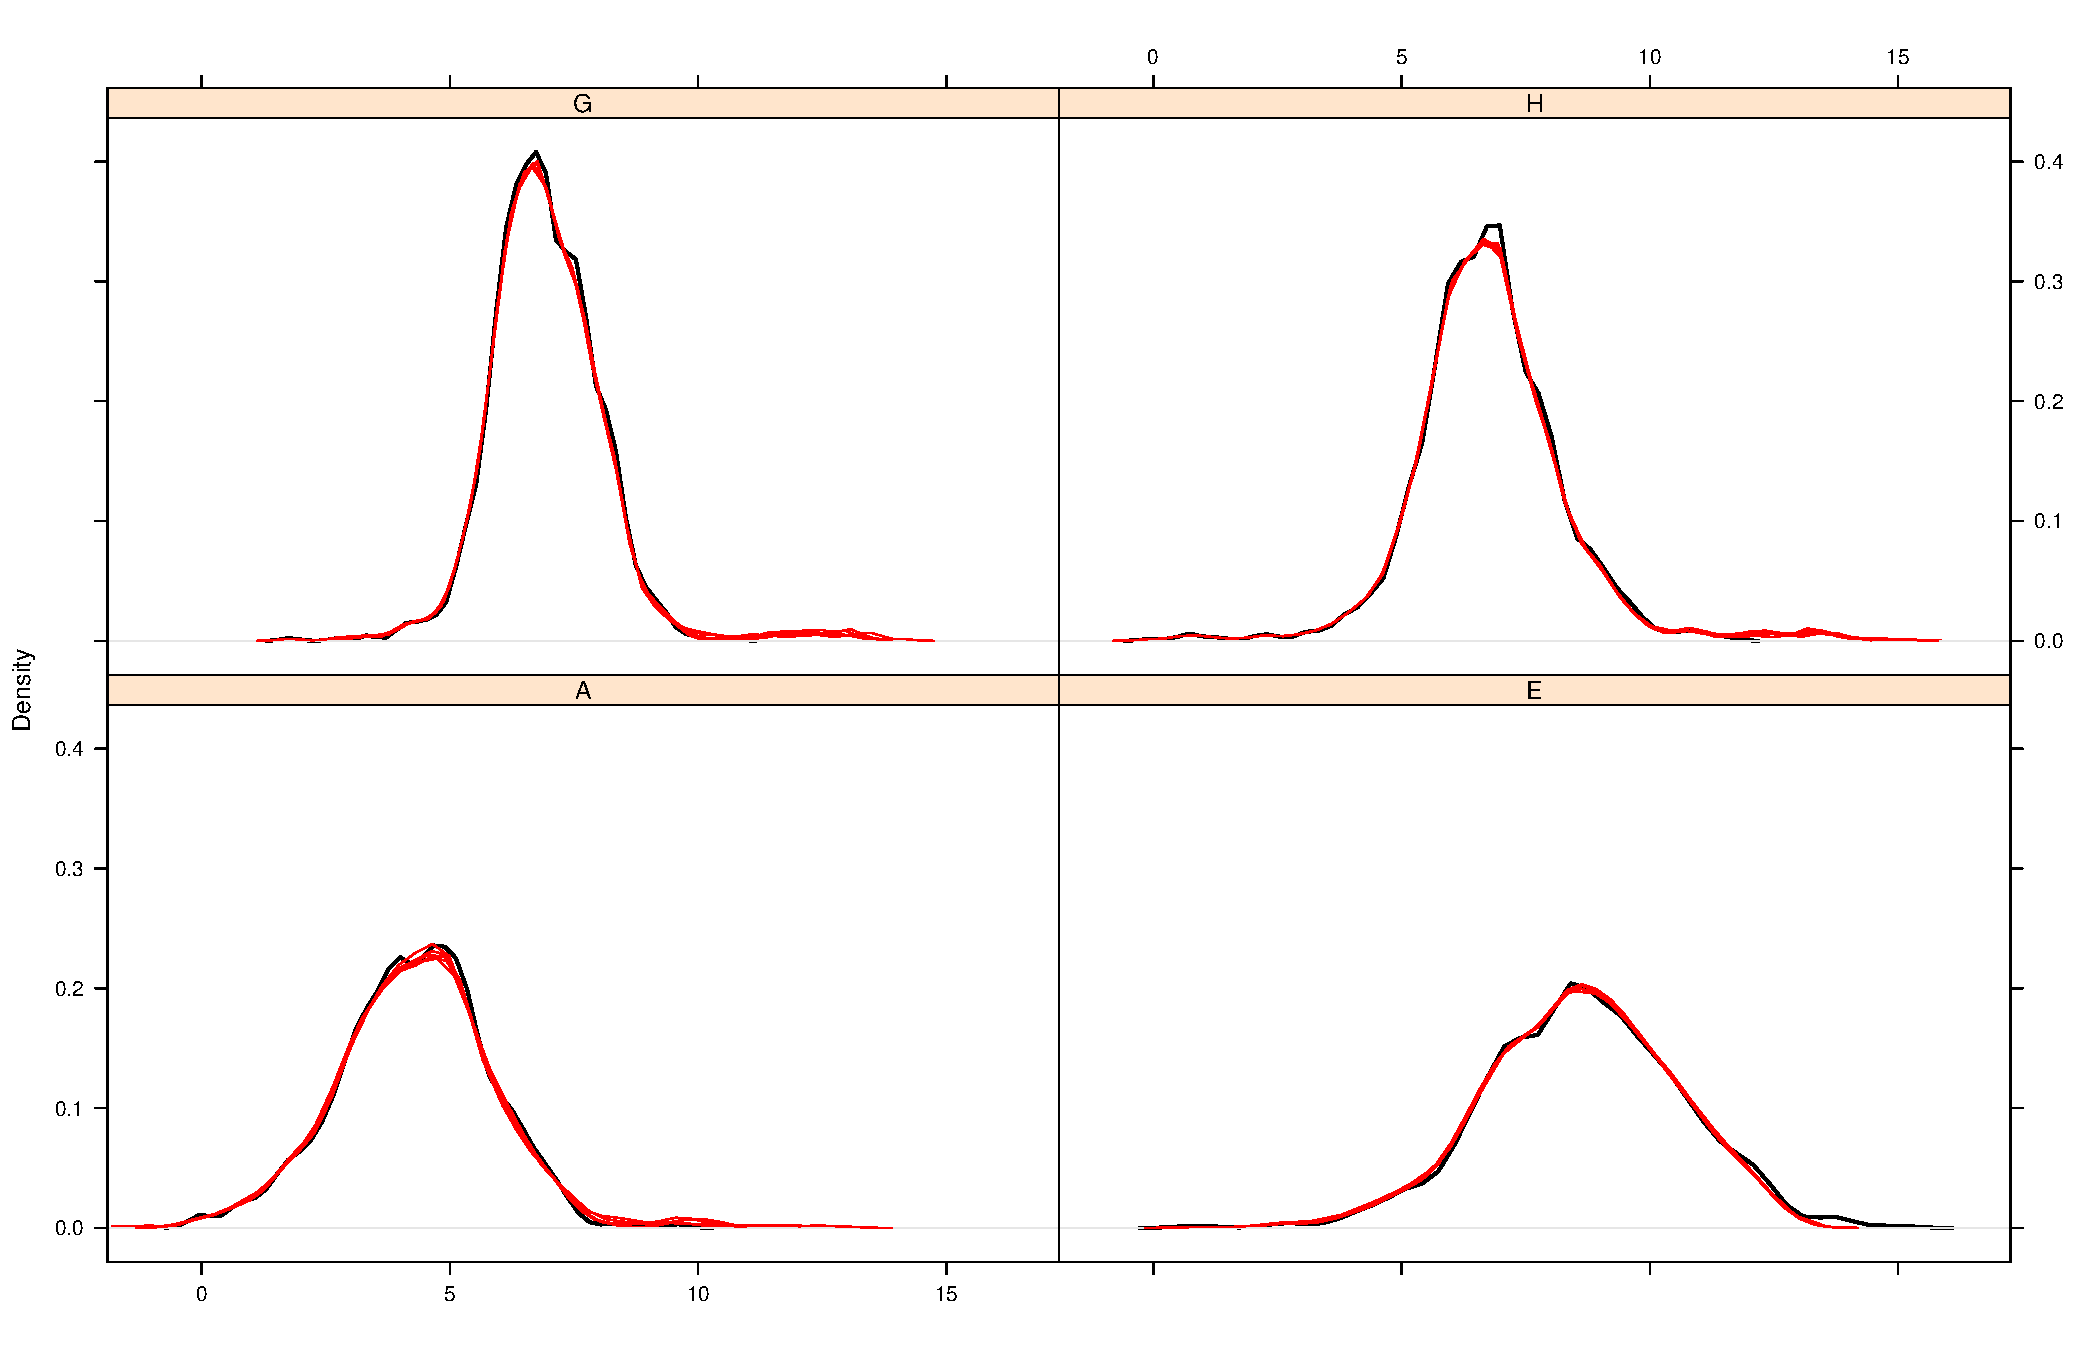
\includegraphics[scale=.3]{plotdens.pdf}
 \end{frame}
 
 \begin{frame}
   \frametitle{TO SUM UP / TO DO}
 PRM emerges as a very effective imputation approach for intricately nested compositional data
 \begin{itemize}
 \item Skewed semicontinuous (or zero-inflated) data 
 \item No need for transformations of the data
 \item No need for post-hoc fixes to handle zeros
 \item Flexibility of mice-based approaches
 \item Works also when all components are missing
 \end{itemize}
 \vspace{.15 in}
 However, the top-level compositional total needs to be observed (or imputed beforehand)
 \newline \\
 A comparison with imputation approaches for single compositions needs to be made
 \end{frame}

\end{document}
